\documentclass[../main.tex]{subfiles}

\firstpageheader{6.042}{Recitation Problems 11}{Page \thepage\ of \numpages}
\runningheader{6.042}{Recitation Problems 11}{Page \thepage\ of \numpages}

\begin{document}

\begin{questions}

  \question Give a description of the equivalence classes associated with each of the following equivalence relations.
  \begin{parts}
    \part Integers $x$ and $y$ are equivalent if $x \equiv y$ (mod 3).
    \begin{solution}

      \{ $n\ |\ (n \in \mathbb{Z}.\ 3|n)$ \} = \{ ..., -6, -3, 0, 3, 6, ... \}

      \{ $n\ |\ (n \in \mathbb{Z}.\ 3|n+1)$ \} = \{ ..., -5, -2, 1, 4, 7, ... \}

      \{ $n\ |\ (n \in \mathbb{Z}.\ 3|n+2)$ \} = \{ ..., -4, -1, 2, 5, 8, ... \}
    \end{solution}

    \part Real numbers $x$ and $y$ are equivalent if $\lceil x \rceil = \lceil y \rceil$, where $\lceil z \rceil$ denotes the smalles integer greater than or equal to $z$.
    \begin{solution}
      The equivalence classes are the intervals $(n,\ n+1]$ for $n \in \mathbb{Z}$.
    \end{solution}
  \end{parts}

  \question Show that neither of the following relations is an equivalence relation by identifying a missing property (reflexivity, symmetry, transitivity). 
  \begin{parts}
    \part The "divides" relation on the positive integers.
    \begin{solution}
      The relation is not symmetric. For example, $3|6$ is true, but $6|3$ is not.
    \end{solution}

    \part The "implies" relation on propositional formulas.
    \begin{solution}
      The relation is not symmetric. For example $false \implies true$, but not $true \implies false$.
    \end{solution}
  \end{parts}

  \pagebreak
  \question MIT Courses
  \begin{parts}
    \part Draw a Hasse diagram for the corresponding partially-ordered set.
    \begin{solution}
    
      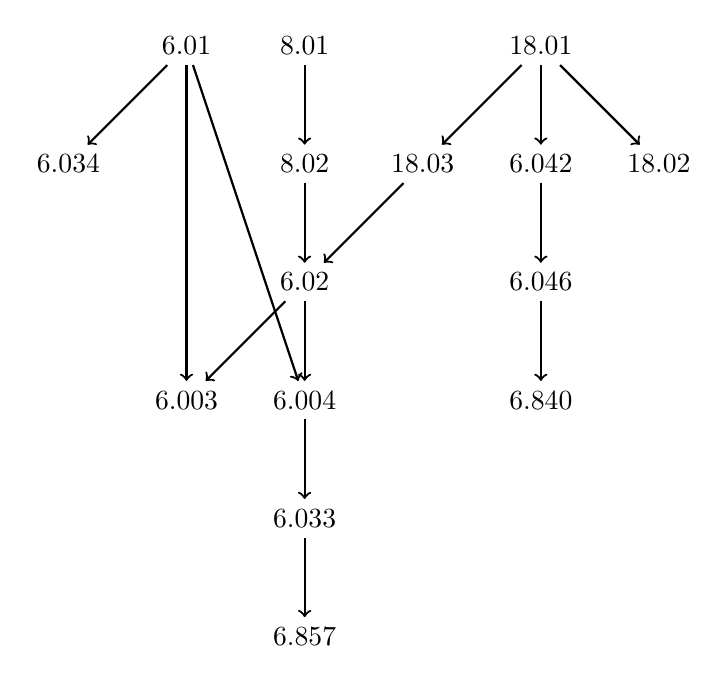
\begin{tikzpicture}[node distance={15mm}, thick] 

        \node (EM1) {}; 
        \node (6_01) [right of=EM1] {$6.01$}; 
        \node (6_034) [below of=EM1] {$6.034$}; 

        \node (8_01) [right of=6_01] {$8.01$}; 
        \node (EM2) [right of=8_01] {}; 
        \node (8_02) [below of=8_01] {$8.02$}; 
        \node (6_02) [below of=8_02] {$6.02$}; 
        \node (6_004) [below of=6_02] {$6.004$}; 
        \node (6_003) [left of=6_004] {$6.003$}; 
        \node (6_033) [below of=6_004] {$6.033$}; 
        \node (6_857) [below of=6_033] {$6.857$}; 

        \node (18_01) [right of=EM2] {$18.01$}; 
        \node (6_042) [below of=18_01] {$6.042$}; 
        \node (18_03) [left of=6_042] {$18.03$}; 
        \node (6_046) [below of=6_042] {$6.046$}; 
        \node (6_840) [below of=6_046] {$6.840$}; 
        \node (18_02) [right of=6_042] {$18.02$}; 

        \draw[->] (8_01) to (8_02);
        \draw[->] (8_02) to (6_02);
        \draw[->] (6_02) to (6_004);
        \draw[->] (6_004) to (6_033);
        \draw[->] (6_033) to (6_857);

        \draw[->] (6_01) to (6_004);
        \draw[->] (6_01) to (6_003);
        \draw[->] (6_01) to (6_034);
        \draw[->] (6_02) to (6_003);

        \draw[->] (18_01) to (18_03);
        \draw[->] (18_01) to (18_02);
        \draw[->] (18_03) to (6_02);
        \draw[->] (18_01) to (6_042);
        \draw[->] (6_042) to (6_046);
        \draw[->] (6_046) to (6_840);

      \end{tikzpicture}
    \end{solution}

    \part Identify a largest chain.
    \begin{solution}
      $8.01 \preceq 8.02 \preceq 6.02 \preceq 6.004 \preceq 6.033 \preceq 6.857$
    \end{solution}

    \part Suppose you want to take all the courses. What is the minimum number of terms required to graduate, if you can take as many courses as you want per term?
    \begin{solution}
      $6$ terms (length of largest chain).
    \end{solution}

    \part Identify a largest antichain.
    \begin{solution}
    $A=$ \{ 6.034, 8.02, 18.03, 6.042, 18.02 \}
    \end{solution}

    \part What is the maximum number of classes that you could possibly take at once?
    \begin{solution}
      $5$ (length of largest antichain).
    \end{solution}

    \part Identify a topological sort of the clases.
    \begin{solution}
      (6.01, 6.034, 8.01, 8.02, 18.01, 18.03, 6.02, 6.003, 6.004, 6.033, 6.857, 6.042, 6.046, 6.840, 18.02)
    \end{solution}

    \part Suppose that you want to take all of the courses, but can handle only two per term. How many terms are required to graduate?
    \begin{solution}

      It takes $8$ terms:

      1. (6.01, 8.01) \\
      2. (18.01, 8.02) \\
      3. (18.03, 18.02) \\
      4. (6.02, 6.042) \\
      5. (6.003, 6.004) \\
      6. (6.033, 6.046) \\
      7. (6.034, 6.840) \\
      8. (6.857)
    \end{solution}

    \part What if you could take three courses per term?
    \begin{solution}
      It takes $6$ terms:
        
      1. (6.01, 8.01, 18.01) \\
      2. (6.034, 8.02, 18.03) \\
      3. (6.02, 6.042, 18.02) \\
      4. (6.003, 4.004, 6.046) \\
      5. (6.033, 6.840) \\
      6. (6.857)
    \end{solution}

    \part Stanford's computer science department offers $n$ courses, limits students to at most $k$ classes per term, and has its own complicated prerequisite structure. De scribe two different lower bounds on the number of terms required to complete all the courses. One should be based on your answers to parts (b) and (c) and a second should be based on your answer to part (g).
    \begin{solution}

      One lower bound is the length of the longest chain.

      Another lower bound is $\lceil \frac{n}{k} \rceil$.
    \end{solution}
  \end{parts}

\end{questions}
\end{document}
